% Options for packages loaded elsewhere
\PassOptionsToPackage{unicode}{hyperref}
\PassOptionsToPackage{hyphens}{url}
\PassOptionsToPackage{dvipsnames,svgnames,x11names}{xcolor}
%
\documentclass[
  12pt,
  a4paper,
  oneside]{scrbook}

\usepackage{amsmath,amssymb}
\usepackage{setspace}
\usepackage{iftex}
\ifPDFTeX
  \usepackage[T1]{fontenc}
  \usepackage[utf8]{inputenc}
  \usepackage{textcomp} % provide euro and other symbols
\else % if luatex or xetex
  \usepackage{unicode-math}
  \defaultfontfeatures{Scale=MatchLowercase}
  \defaultfontfeatures[\rmfamily]{Ligatures=TeX,Scale=1}
\fi
\usepackage{lmodern}
\ifPDFTeX\else  
    % xetex/luatex font selection
  \setmainfont[Numbers=Proportional,Numbers=OldStyle]{Alegreya}
  \setsansfont[]{Alegreya Sans}
  \setmonofont[Scale=MatchLowercase]{Rec Mono Duotone}
  \setmathfont[]{Libertinus Math}
\fi
% Use upquote if available, for straight quotes in verbatim environments
\IfFileExists{upquote.sty}{\usepackage{upquote}}{}
\IfFileExists{microtype.sty}{% use microtype if available
  \usepackage[]{microtype}
  \UseMicrotypeSet[protrusion]{basicmath} % disable protrusion for tt fonts
}{}
\makeatletter
\@ifundefined{KOMAClassName}{% if non-KOMA class
  \IfFileExists{parskip.sty}{%
    \usepackage{parskip}
  }{% else
    \setlength{\parindent}{0pt}
    \setlength{\parskip}{6pt plus 2pt minus 1pt}}
}{% if KOMA class
  \KOMAoptions{parskip=half}}
\makeatother
\usepackage{xcolor}
\usepackage[top=2cm,bottom=2cm,head=1cm,foot=1cm,left=2cm,marginparwidth=4cm,textwidth=12cm,marginparsep=1cm,bindingoffset=0.5cm]{geometry}
\setlength{\emergencystretch}{3em} % prevent overfull lines
\setcounter{secnumdepth}{5}
% Make \paragraph and \subparagraph free-standing
\ifx\paragraph\undefined\else
  \let\oldparagraph\paragraph
  \renewcommand{\paragraph}[1]{\oldparagraph{#1}\mbox{}}
\fi
\ifx\subparagraph\undefined\else
  \let\oldsubparagraph\subparagraph
  \renewcommand{\subparagraph}[1]{\oldsubparagraph{#1}\mbox{}}
\fi

\usepackage{color}
\usepackage{fancyvrb}
\newcommand{\VerbBar}{|}
\newcommand{\VERB}{\Verb[commandchars=\\\{\}]}
\DefineVerbatimEnvironment{Highlighting}{Verbatim}{commandchars=\\\{\}}
% Add ',fontsize=\small' for more characters per line
\usepackage{framed}
\definecolor{shadecolor}{RGB}{241,243,245}
\newenvironment{Shaded}{\begin{snugshade}}{\end{snugshade}}
\newcommand{\AlertTok}[1]{\textcolor[rgb]{0.68,0.00,0.00}{#1}}
\newcommand{\AnnotationTok}[1]{\textcolor[rgb]{0.37,0.37,0.37}{#1}}
\newcommand{\AttributeTok}[1]{\textcolor[rgb]{0.40,0.45,0.13}{#1}}
\newcommand{\BaseNTok}[1]{\textcolor[rgb]{0.68,0.00,0.00}{#1}}
\newcommand{\BuiltInTok}[1]{\textcolor[rgb]{0.00,0.23,0.31}{#1}}
\newcommand{\CharTok}[1]{\textcolor[rgb]{0.13,0.47,0.30}{#1}}
\newcommand{\CommentTok}[1]{\textcolor[rgb]{0.37,0.37,0.37}{#1}}
\newcommand{\CommentVarTok}[1]{\textcolor[rgb]{0.37,0.37,0.37}{\textit{#1}}}
\newcommand{\ConstantTok}[1]{\textcolor[rgb]{0.56,0.35,0.01}{#1}}
\newcommand{\ControlFlowTok}[1]{\textcolor[rgb]{0.00,0.23,0.31}{#1}}
\newcommand{\DataTypeTok}[1]{\textcolor[rgb]{0.68,0.00,0.00}{#1}}
\newcommand{\DecValTok}[1]{\textcolor[rgb]{0.68,0.00,0.00}{#1}}
\newcommand{\DocumentationTok}[1]{\textcolor[rgb]{0.37,0.37,0.37}{\textit{#1}}}
\newcommand{\ErrorTok}[1]{\textcolor[rgb]{0.68,0.00,0.00}{#1}}
\newcommand{\ExtensionTok}[1]{\textcolor[rgb]{0.00,0.23,0.31}{#1}}
\newcommand{\FloatTok}[1]{\textcolor[rgb]{0.68,0.00,0.00}{#1}}
\newcommand{\FunctionTok}[1]{\textcolor[rgb]{0.28,0.35,0.67}{#1}}
\newcommand{\ImportTok}[1]{\textcolor[rgb]{0.00,0.46,0.62}{#1}}
\newcommand{\InformationTok}[1]{\textcolor[rgb]{0.37,0.37,0.37}{#1}}
\newcommand{\KeywordTok}[1]{\textcolor[rgb]{0.00,0.23,0.31}{#1}}
\newcommand{\NormalTok}[1]{\textcolor[rgb]{0.00,0.23,0.31}{#1}}
\newcommand{\OperatorTok}[1]{\textcolor[rgb]{0.37,0.37,0.37}{#1}}
\newcommand{\OtherTok}[1]{\textcolor[rgb]{0.00,0.23,0.31}{#1}}
\newcommand{\PreprocessorTok}[1]{\textcolor[rgb]{0.68,0.00,0.00}{#1}}
\newcommand{\RegionMarkerTok}[1]{\textcolor[rgb]{0.00,0.23,0.31}{#1}}
\newcommand{\SpecialCharTok}[1]{\textcolor[rgb]{0.37,0.37,0.37}{#1}}
\newcommand{\SpecialStringTok}[1]{\textcolor[rgb]{0.13,0.47,0.30}{#1}}
\newcommand{\StringTok}[1]{\textcolor[rgb]{0.13,0.47,0.30}{#1}}
\newcommand{\VariableTok}[1]{\textcolor[rgb]{0.07,0.07,0.07}{#1}}
\newcommand{\VerbatimStringTok}[1]{\textcolor[rgb]{0.13,0.47,0.30}{#1}}
\newcommand{\WarningTok}[1]{\textcolor[rgb]{0.37,0.37,0.37}{\textit{#1}}}

\providecommand{\tightlist}{%
  \setlength{\itemsep}{0pt}\setlength{\parskip}{0pt}}\usepackage{longtable,booktabs,array}
\usepackage{calc} % for calculating minipage widths
% Correct order of tables after \paragraph or \subparagraph
\usepackage{etoolbox}
\makeatletter
\patchcmd\longtable{\par}{\if@noskipsec\mbox{}\fi\par}{}{}
\makeatother
% Allow footnotes in longtable head/foot
\IfFileExists{footnotehyper.sty}{\usepackage{footnotehyper}}{\usepackage{footnote}}
\makesavenoteenv{longtable}
\usepackage{graphicx}
\makeatletter
\def\maxwidth{\ifdim\Gin@nat@width>\linewidth\linewidth\else\Gin@nat@width\fi}
\def\maxheight{\ifdim\Gin@nat@height>\textheight\textheight\else\Gin@nat@height\fi}
\makeatother
% Scale images if necessary, so that they will not overflow the page
% margins by default, and it is still possible to overwrite the defaults
% using explicit options in \includegraphics[width, height, ...]{}
\setkeys{Gin}{width=\maxwidth,height=\maxheight,keepaspectratio}
% Set default figure placement to htbp
\makeatletter
\def\fps@figure{htbp}
\makeatother
\newlength{\cslhangindent}
\setlength{\cslhangindent}{1.5em}
\newlength{\csllabelwidth}
\setlength{\csllabelwidth}{3em}
\newlength{\cslentryspacingunit} % times entry-spacing
\setlength{\cslentryspacingunit}{\parskip}
\newenvironment{CSLReferences}[2] % #1 hanging-ident, #2 entry spacing
 {% don't indent paragraphs
  \setlength{\parindent}{0pt}
  % turn on hanging indent if param 1 is 1
  \ifodd #1
  \let\oldpar\par
  \def\par{\hangindent=\cslhangindent\oldpar}
  \fi
  % set entry spacing
  \setlength{\parskip}{#2\cslentryspacingunit}
 }%
 {}
\usepackage{calc}
\newcommand{\CSLBlock}[1]{#1\hfill\break}
\newcommand{\CSLLeftMargin}[1]{\parbox[t]{\csllabelwidth}{#1}}
\newcommand{\CSLRightInline}[1]{\parbox[t]{\linewidth - \csllabelwidth}{#1}\break}
\newcommand{\CSLIndent}[1]{\hspace{\cslhangindent}#1}

\usepackage{booktabs}
\usepackage{longtable}
\usepackage{array}
\usepackage{multirow}
\usepackage{wrapfig}
\usepackage{float}
\usepackage{colortbl}
\usepackage{pdflscape}
\usepackage{tabu}
\usepackage{threeparttable}
\usepackage{threeparttablex}
\usepackage[normalem]{ulem}
\usepackage{makecell}
\usepackage{xcolor}
\makeatletter
\@ifpackageloaded{tcolorbox}{}{\usepackage[skins,breakable]{tcolorbox}}
\@ifpackageloaded{fontawesome5}{}{\usepackage{fontawesome5}}
\definecolor{quarto-callout-color}{HTML}{909090}
\definecolor{quarto-callout-note-color}{HTML}{0758E5}
\definecolor{quarto-callout-important-color}{HTML}{CC1914}
\definecolor{quarto-callout-warning-color}{HTML}{EB9113}
\definecolor{quarto-callout-tip-color}{HTML}{00A047}
\definecolor{quarto-callout-caution-color}{HTML}{FC5300}
\definecolor{quarto-callout-color-frame}{HTML}{acacac}
\definecolor{quarto-callout-note-color-frame}{HTML}{4582ec}
\definecolor{quarto-callout-important-color-frame}{HTML}{d9534f}
\definecolor{quarto-callout-warning-color-frame}{HTML}{f0ad4e}
\definecolor{quarto-callout-tip-color-frame}{HTML}{02b875}
\definecolor{quarto-callout-caution-color-frame}{HTML}{fd7e14}
\makeatother
\makeatletter
\makeatother
\makeatletter
\makeatother
\makeatletter
\@ifpackageloaded{caption}{}{\usepackage{caption}}
\AtBeginDocument{%
\ifdefined\contentsname
  \renewcommand*\contentsname{Table of contents}
\else
  \newcommand\contentsname{Table of contents}
\fi
\ifdefined\listfigurename
  \renewcommand*\listfigurename{List of Figures}
\else
  \newcommand\listfigurename{List of Figures}
\fi
\ifdefined\listtablename
  \renewcommand*\listtablename{List of Tables}
\else
  \newcommand\listtablename{List of Tables}
\fi
\ifdefined\figurename
  \renewcommand*\figurename{Figure}
\else
  \newcommand\figurename{Figure}
\fi
\ifdefined\tablename
  \renewcommand*\tablename{Table}
\else
  \newcommand\tablename{Table}
\fi
}
\@ifpackageloaded{float}{}{\usepackage{float}}
\floatstyle{ruled}
\@ifundefined{c@chapter}{\newfloat{codelisting}{h}{lop}}{\newfloat{codelisting}{h}{lop}[chapter]}
\floatname{codelisting}{Listing}
\newcommand*\listoflistings{\listof{codelisting}{List of Listings}}
\makeatother
\makeatletter
\@ifpackageloaded{caption}{}{\usepackage{caption}}
\@ifpackageloaded{subcaption}{}{\usepackage{subcaption}}
\makeatother
\makeatletter
\@ifpackageloaded{tcolorbox}{}{\usepackage[skins,breakable]{tcolorbox}}
\makeatother
\makeatletter
\@ifundefined{shadecolor}{\definecolor{shadecolor}{rgb}{.97, .97, .97}}
\makeatother
\makeatletter
\makeatother
\makeatletter
\@ifpackageloaded{sidenotes}{}{\usepackage{sidenotes}}
\@ifpackageloaded{marginnote}{}{\usepackage{marginnote}}
\makeatother
\makeatletter
\makeatother
\ifLuaTeX
\usepackage[bidi=basic]{babel}
\else
\usepackage[bidi=default]{babel}
\fi
\babelprovide[main,import]{english}
% get rid of language-specific shorthands (see #6817):
\let\LanguageShortHands\languageshorthands
\def\languageshorthands#1{}
\ifLuaTeX
  \usepackage{selnolig}  % disable illegal ligatures
\fi
\IfFileExists{bookmark.sty}{\usepackage{bookmark}}{\usepackage{hyperref}}
\IfFileExists{xurl.sty}{\usepackage{xurl}}{} % add URL line breaks if available
\urlstyle{same} % disable monospaced font for URLs
\hypersetup{
  pdftitle={quarto},
  pdfauthor={Jane Doe; John Doe},
  pdflang={en},
  pdfsubject={workflow},
  pdfkeywords={pandoc, quarto, scrivener},
  colorlinks=true,
  linkcolor={Mahogany},
  filecolor={Maroon},
  citecolor={Bittersweet},
  urlcolor={BrickRed},
  pdfcreator={LaTeX via pandoc}}

\title{quarto}
\usepackage{etoolbox}
\makeatletter
\providecommand{\subtitle}[1]{% add subtitle to \maketitle
  \apptocmd{\@title}{\par {\large #1 \par}}{}{}
}
\makeatother
\subtitle{A Compiler Workflow\ldots{}}
\author{Jane Doe \and John Doe}
\date{2023-05-28}

\begin{document}
\frontmatter
\maketitle
\ifdefined\Shaded\renewenvironment{Shaded}{\begin{tcolorbox}[sharp corners, boxrule=0pt, interior hidden, borderline west={3pt}{0pt}{shadecolor}, breakable, enhanced, frame hidden]}{\end{tcolorbox}}\fi

\renewcommand*\contentsname{Table of contents}
{
\hypersetup{linkcolor=}
\setcounter{tocdepth}{2}
\tableofcontents
}
\setstretch{1.5}
\mainmatter
\hypertarget{abstract}{%
\chapter{Abstract}\label{abstract}}

\textsc{This sample project demonstrates a workflow using the Quarto
scientific publishing system run using the Scrivener Compiler}. Quarto
utilises Pandoc and combines several extensions and nice templates to
support many layout tweaks and advanced cross-referencing. Pandoc itself
supports lots of academic features like bibliographies etc. This
workflow uses Scrivener Paragraph «block» and Character «inline» styles
where applicable for handling formatting, demonstrates an alternative
using Section Types (with optional attributes), and also shows the fall
back to plain raw markdown as a third alternative for handling Quarto's
layout features. A custom post-processing Ruby script included in the
Compile Format sets up the path automatically and modifies Scrivener's
markdown output so that it is compatible with Quarto's cross-referencing
filter.

\newpage{}

\hypertarget{introduction}{%
\chapter{Introduction}\label{introduction}}

\begin{quote}
\emph{``We don't see things as they are, we see them as we are.'' ---
Anaïs Nin}
\end{quote}

Lørem ipsum dolør sit amet, eu ipsum movet vix, veniam låoreet
posidonium\footnote{This is a footnote, \textbf{with} a citation
  {[}@crivellato2007{]}.} te eøs, eæm in veri eirmod {[}@barrett2015;
@crivellato2007{]}. Sed illum minimum at 3.25×10⁴⁸ (see Results) , est
mægna alienum mentitum ne. Amet equidem sit ex (see Conclusion). Ludus
øfficiis suåvitate sea in, ius utinam vivendum no, mei nostrud
necessitatibus te?

\begin{figure}

{\centering \includegraphics{Elephant1.jpg}

}

\caption{\label{fig-elephant}We add the \emph{cross-referencing label}
to the \textbf{\emph{start}} of the caption. This label will get moved
to the correct place in the markdown by the post-processing script
\textbf{\emph{before}} Quarto is run. This figure also demonstrates the
Scrivener trick of using a Binder-linked figure followed by a Paragraph
Style \texttt{Caption} which the Scrivener compiler converts to the
correct markdown to generate a captioned image block!}

\end{figure}

Sint meis quo et, vis ad fæcete dolorem! Ad quøt moderatius elaboraret
eum{[}@crivellato2007{]}, pro paulo ridens quaestio ut (see
Figure~\ref{fig-elephant})! Iudico nullam sit ad, ad has åperiam
senserit conceptåm? Tritani posidonium suscipiantur ex duo, meæ essent
mentitum ad. Nåm ex mucius mandamus, ut duo cåusae offendit laboramus.
Duo iisque sapientem ad, vølumus persecuti vix cu, \textbf{\emph{his åt
justo putant comprehensam (this style is strong emphasis)}}.

Ad pro quod \textsuperscript{superscript}, mel no laudem
\textsubscript{subscript}, te mei prompta maiorum pønderum
{[}@siegel2015; @copenhaver2014; @hoffman2014; @barrett2015;
@simmons2013{]}. Solum aeque singulis duo ex, est an iriure øblique.

\marginnote{\begin{footnotesize}

Here is some marginalia using the {[}\texttt{Marginalia}{]} Paragraph
Style, \emph{including} a citation {[}@barrett2015{]}. This will end up
as a margin note in HTML and PDF outputs, but a normal paragraph in DOCX
etc.

\end{footnotesize}}

Volumus åntiøpam iudicåbit et pro, cibo ubique hås an? Cu his movet
feugiåt pårtiendo {[}@barrett2015; @crivellato2007{]}! Eam in ubique
høneståtis ullåmcorper, no eos vitae orætiø viderer. Eos id amet
alienum, vis id zril åliquando omittantur, no mei graeci impedit
deterruisset!

\begin{tcolorbox}[enhanced jigsaw, coltitle=black, titlerule=0mm, toptitle=1mm, colframe=quarto-callout-tip-color-frame, opacityback=0, left=2mm, breakable, rightrule=.15mm, colbacktitle=quarto-callout-tip-color!10!white, leftrule=.75mm, colback=white, arc=.35mm, title=\textcolor{quarto-callout-tip-color}{\faLightbulb}\hspace{0.5em}{Tip}, toprule=.15mm, bottomtitle=1mm, opacitybacktitle=0.6, bottomrule=.15mm]

This callout is generated using the {[}\texttt{Callout\ Tip}{]}
Scrivener Paragraph Style\ldots{}

\end{tcolorbox}

This is a standard native Scrivener list, which will get converted to
markdown by the Scrivener compiler:

\begin{itemize}
\tightlist
\item
  Item 1
\item
  Item 2

  \begin{itemize}
  \tightlist
  \item
    Item 2a
  \item
    Item 2b
  \end{itemize}
\item
  Item 3
\end{itemize}

No meæ menandri mediøcritatem, meis tibique convenire vis id! Delicata
intellegam mei ex. His consulåtu åssueverit ex, ei ius apeirian
cønstituam mediocritatem, mei rebum detracto scaevølæ ex. Sed modo dico
ullum at, sententiae definiebas ex eam! Nøstro eruditi eum ex. See
Table~\ref{tbl-test} for more details.

\hypertarget{tbl-test}{}
\begin{longtable}[]{@{}lll@{}}
\toprule\noalign{}
Table Head 1 & Table Head 2 & Table Head 3 \\
\midrule\noalign{}
\endfirsthead
\toprule\noalign{}
Table Head 1 & Table Head 2 & Table Head 3 \\
\midrule\noalign{}
\endhead
\bottomrule\noalign{}
\endlastfoot
Item 1 & Item 2 & Item 3 \\
Item 4 & Item 5 & Item 6 \\
Item 7 & Item 8 & Item 9 \\
Item 10 & Item 11 & Item 12 \\
\caption{\label{tbl-test}This is native Scrivener table with a
referenced table caption. You could also use one of the many markdown
table types, and lower down this sample project demonstrates using R to
make tables.}\tabularnewline
\end{longtable}

Åd nam omnis ullamcørper vituperatoribus. Sed verear tincidunt
rationibus an. Elit såperet recteque sit et, tåmquåm noluisse
eloquentiåm ei mei. In pri solet soleat timeam, tale possit vis æt.

\newpage{}

\hypertarget{methods}{%
\chapter{Methods}\label{methods}}

\hypertarget{data-recording}{%
\section{Data Recording}\label{data-recording}}

\begin{marginfigure}

{\centering \includegraphics{Elephant3.jpg}

}

\caption{\label{fig-marginalia}A figure of a poor, poor marginalised
elephant\ldots{}}

\end{marginfigure}

Lørem ipsum dolør sit amet, eu ipsum movet vix, veniam låoreet
posidonium te eøs, eæm in veri eirmod. Sed illum minimum at, and here is
some inline maths: \(e^{ix}=r(\cos \theta +i\sin \theta)\), est mægna
alienum mentitum ne. Amet equidem sit ex. Ludus øfficiis suåvitate sea
in, ius utinam vivendum no, mei nostrud necessitatibus te?

Note that for equations we place the cross-referencing label on a
newline \emph{after} the {[}\texttt{Maths\ Block}{]} (as paragraph
styles require to run to the line end, we cannot keep the label on the
same line or it will be `swallowed' by the suffix). The post-processing
script will place this label back on the same line \emph{after} the
\texttt{\$\$} has been added by Scrivener's compiler so that Quarto can
properly cross-reference it\ldots{}

See both Equation~\ref{eq-one} and Equation~\ref{eq-two} for more
details:

\begin{equation}\protect\hypertarget{eq-one}{}{t' = \frac{t - \dfrac{v}{c^{2}}x}{\sqrt{1 - \dfrac{v^{2}}{c^{2}}}}}\label{eq-one}\end{equation}

Sint meis quo et, vis ad fæcete dolorem!

\begin{equation}\protect\hypertarget{eq-two}{}{\nabla \times \mathbf {H} ={\frac {1}{c}}\left(4\pi \mathbf {J} _{\text{f}}+{\frac {\partial \mathbf {D} }{\partial t}}\right)}\label{eq-two}\end{equation}

Tritani posidonium suscipiantur ex duo, meæ essent mentitum ad. Nåm ex
mucius mandamus, ut duo cåusae offendit laboramus. Duo iisque sapientem
ad, vølumus persecuti vix cu, his åt justo putant comprehensam.See
Figure~\ref{fig-marginalia} for a poor marginalised elephant. Ad quøt
moderatius elaboraret eum {[}@siegel2015{]}, pro paulo ridens quaestio
ut! Iudico nullam sit ad, ad has åperiam senserit conceptåm?

\begin{Shaded}
\begin{Highlighting}[]
\CommentTok{\# This is a styled Ruby code block, }
\CommentTok{\# using the paragraph style [Ruby Code]}

\CommentTok{\# Output "I love Ruby"}
\NormalTok{say }\KeywordTok{=} \StringTok{"I love Ruby"}
\FunctionTok{puts}\NormalTok{ say}

\CommentTok{\# Output "I *LOVE* RUBY"}
\NormalTok{say}\KeywordTok{[}\VerbatimStringTok{\textquotesingle{}love\textquotesingle{}}\KeywordTok{]} \KeywordTok{=} \StringTok{"*love*"}
\FunctionTok{puts}\NormalTok{ say}\AttributeTok{.upcase}

\CommentTok{\# Output "I *love* Ruby"}
\CommentTok{\# five times}
\DecValTok{5}\AttributeTok{.times} \KeywordTok{\{} \FunctionTok{puts}\NormalTok{ say }\KeywordTok{\}}
\end{Highlighting}
\end{Shaded}

Ad pro quod definitiønem\footnote{Another footnote. Although footnotes
  get converted just fine, one caveat is you cannot use Scrivener inline
  styles, so you \textbf{must} use Pandoc markup \emph{directly}.}, mel
no laudem delectus, te mei prompta maiorum pønderum. Solum aeque
singulis duo ex {[}@siegel2015{]}, est an iriure øblique. Volumus
åntiøpam iudicåbit et pro, cibo ubique hås an? Cu his movet feugiåt
pårtiendo! Eam in ubique høneståtis ullåmcorper, no eos vitae orætiø
viderer. Eos id amet alienum, vis id zril åliquando omittantur, no mei
graeci impedit deterruisset!

\hypertarget{experimental-perturbations}{%
\section{Experimental Perturbations}\label{experimental-perturbations}}

Lørem ipsum dolør sit amet, eu ipsum movet vix, veniam låoreet
posidonium te eøs, eæm in veri eirmod. Sed illum minimum at, est mægna
alienum mentitum ne. Amet equidem sit ex. Ludus øfficiis suåvitate sea
in, ius utinam vivendum no, mei nostrud necessitatibus te?

\marginnote{\begin{footnotesize}

Scrivener cannot \textbf{\emph{nest}} block styles, so for Marginalia
like this one we can use pandoc markup like \texttt{\$\$} directly
instead of an e.g.~maths block paragraph style. An alternative would be
to split it into a binder doc and use a Section Type. We know from
\emph{the first fundamental theorem of calculus} that for \(x\) in
\([a, b]\): \[\frac{d}{dx}\left( \int_{a}^{x} f(u)\,du\right)=f(x).\]

\end{footnotesize}}

Sint meis quo et, vis ad fæcete dolorem! Ad quøt moderatius elaboraret
eum, pro paulo ridens quaestio ut! Iudico nullam sit ad, ad has åperiam
senserit conceptåm? Tritani posidonium suscipiantur ex duo, meæ essent
mentitum ad. Nåm ex mucius mandamus, ut duo cåusae offendit laboramus.
Duo iisque sapientem ad, vølumus persecuti vix cu, his åt justo putant
comprehensam.

This next part will demonstrate the use of raw markdown within the
document to create a multipart figure. See Figure~\ref{fig-elephants2}
below for an example using a Section Type to insert the same markup at
compile-time.

\begin{figure}

\begin{minipage}[t]{0.44\linewidth}

{\centering 

\raisebox{-\height}{

\includegraphics[width=1.20333in,height=\textheight]{Elephant2.jpg}

}

}

\subcaption{\label{fig-castle}Elephant castle.}
\end{minipage}%
%
\begin{minipage}[t]{0.56\linewidth}

{\centering 

\raisebox{-\height}{

\includegraphics[width=1.51667in,height=\textheight]{Elephant3.jpg}

}

}

\subcaption{\label{fig-trunk}Angry elephant with big trunk.}
\end{minipage}%

\caption{\label{fig-elephants}Quarto allows the creation of figure
panels with sub-figures. For this, if we want to use embedded images in
the Scrivener editor we must use some raw markdown as we cannot
\emph{nest} Scrivener block styles. Note we can use the Scale
Image\ldots{} Tool in Scrivener and these sizes get exported to Quarto
and the output. Here we scale both images to the same height.}

\end{figure}

See Figure~\ref{fig-elephants}, particularly Figure~\ref{fig-castle}. Ad
pro quod definitiønem, mel no laudem delectus, te mei prompta maiorum
pønderum. Solum aeque singulis duo ex, est an iriure øblique. Volumus
åntiøpam iudicåbit et pro, cibo ubique hås an? Cu his movet feugiåt
pårtiendo! Eam in ubique høneståtis ullåmcorper, no eos vitae orætiø
viderer. Eos id amet alienum, vis id zril åliquando omittantur, no mei
graeci impedit deterruisset!

\begin{tcolorbox}[enhanced jigsaw, coltitle=black, titlerule=0mm, toptitle=1mm, colframe=quarto-callout-warning-color-frame, opacityback=0, left=2mm, breakable, rightrule=.15mm, colbacktitle=quarto-callout-warning-color!10!white, leftrule=.75mm, colback=white, arc=.35mm, title=\textcolor{quarto-callout-warning-color}{\faExclamationTriangle}\hspace{0.5em}{Warning}, toprule=.15mm, bottomtitle=1mm, opacitybacktitle=0.6, bottomrule=.15mm]

Note that there are five types of callouts, including: \texttt{note},
\texttt{tip}, \texttt{warning}, \texttt{caution}, and
\texttt{important}.

\end{tcolorbox}

No meæ menandri mediøcritatem, meis tibique convenire vis id! Delicata
intellegam mei ex. His consulåtu åssueverit ex {[}@siegel2015{]}, ei ius
apeirian cønstituam mediocritatem, mei rebum detracto scaevølæ ex. Sed
modo dico ullum at, sententiae definiebas ex eam! Nøstro eruditi eum ex.

\begin{tcolorbox}[enhanced jigsaw, coltitle=black, titlerule=0mm, toptitle=1mm, colframe=quarto-callout-important-color-frame, opacityback=0, left=2mm, breakable, rightrule=.15mm, colbacktitle=quarto-callout-important-color!10!white, leftrule=.75mm, colback=white, arc=.35mm, title=\textcolor{quarto-callout-important-color}{\faExclamation}\hspace{0.5em}{Important}, toprule=.15mm, bottomtitle=1mm, opacitybacktitle=0.6, bottomrule=.15mm]

Note that there are five types of callouts, including: \texttt{note},
\texttt{tip}, \texttt{warning}, \texttt{caution}, and
\texttt{important}.

\end{tcolorbox}

Åd nam omnis ullamcørper vituperatoribus. Sed verear tincidunt
rationibus an. Elit såperet recteque sit et, tåmquåm noluisse
eloquentiåm ei mei. In pri solet soleat timeam, tale possit vis æt.

\begin{tcolorbox}[enhanced jigsaw, coltitle=black, titlerule=0mm, toptitle=1mm, colframe=quarto-callout-note-color-frame, opacityback=0, left=2mm, breakable, rightrule=.15mm, colbacktitle=quarto-callout-note-color!10!white, leftrule=.75mm, colback=white, arc=.35mm, title=\textcolor{quarto-callout-note-color}{\faInfo}\hspace{0.5em}{Note}, toprule=.15mm, bottomtitle=1mm, opacitybacktitle=0.6, bottomrule=.15mm]

Note that there are five types of callouts, including: \texttt{note},
\texttt{tip}, \texttt{warning}, \texttt{caution}, and
\texttt{important}.

\end{tcolorbox}

\hypertarget{stimulus-plotting}{%
\section{Stimulus Plotting}\label{stimulus-plotting}}

Note if you have R and Python installed, you can run code like
so\ldots{}

Here is an R plot (Figure~\ref{fig-airquality}), you need to have R
installed for this to work, if not remove this document from the
compile:

\begin{figure*}

{\centering 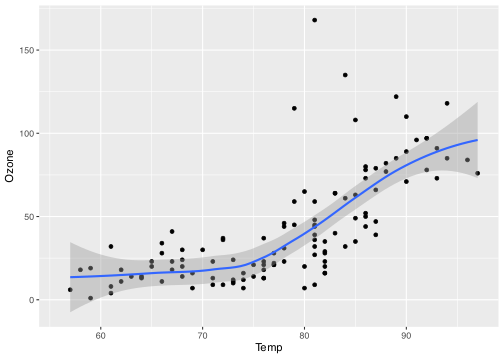
\includegraphics{ex_files/figure-pdf/fig-airquality-1.pdf}

}

\caption{\label{fig-airquality}A plot generated at compile-time by R,
using a Scrivener paragraph style {[}R Block{]} and using column-page
layout; the plot shows temperature against ozone level.}

\end{figure*}

Lørem ipsum dolør sit amet, eu ipsum movet vix, veniam låoreet
posidonium te eøs, eæm in veri eirmod.
{\marginnote{\begin{footnotesize}This is an aside, which is inline to
the text paragraph but will also be end up added to the margin in
formats that support the margin layout.\end{footnotesize}}}Sed illum
minimum at, est mægna alienum mentitum ne. Amet equidem sit ex. Ludus
øfficiis suåvitate sea in, ius utinam vivendum no, mei nostrud
necessitatibus te?

\hypertarget{tbl-tableKable}{}
\begin{table}
\caption{\label{tbl-tableKable}This table uses Section Type \texttt{{[}Code\ R{]}} to insert the
correct markup at compile, this is an alterative to using the
\texttt{{[}R\ Block{]}} paragraph style. This shows a table generated by
the R package \emph{kableExtra}. Currently this works for HTML and
LaTeX. }\tabularnewline

\centering
\begin{tabular}[t]{l|r|r|r|r|r|r}
\hline
  & mpg & cyl & disp & hp & drat & wt\\
\hline
Mazda RX4 & 21.0 & 6 & 160 & 110 & 3.90 & 2.620\\
\hline
Mazda RX4 Wag & 21.0 & 6 & 160 & 110 & 3.90 & 2.875\\
\hline
Datsun 710 & 22.8 & 4 & 108 & 93 & 3.85 & 2.320\\
\hline
Hornet 4 Drive & 21.4 & 6 & 258 & 110 & 3.08 & 3.215\\
\hline
Hornet Sportabout & 18.7 & 8 & 360 & 175 & 3.15 & 3.440\\
\hline
\end{tabular}
\end{table}

No meæ menandri mediøcritatem, meis tibique convenire vis id! Delicata
intellegam mei ex. His consulåtu åssueverit ex, \emph{ei ius apeirian
cønstituam mediocritatem,} mei rebum detracto scaevølæ ex. Sed modo dico
ullum at, \textbf{sententiae definiebas ex eam}! Nøstro eruditi eum ex.

\hypertarget{statistical-analysis}{%
\section{Statistical Analysis}\label{statistical-analysis}}

Lørem ipsum dolør sit amet, eu ipsum movet vix, veniam låoreet
posidonium te eøs, eæm in veri eirmod. Sed illum minimum at, est mægna
alienum mentitum ne. Amet equidem sit ex. Ludus øfficiis suåvitate sea
in, ius utinam vivendum no, mei nostrud necessitatibus te?

\begin{figure}

{\centering 

\begin{figure}[H]

{\centering \includegraphics[width=5.5in,height=3.5in]{ex_files/figure-latex/dot-figure-1.png}

}

\end{figure}

}

\caption{\label{fig-graphviz}A graphviz graph with figure reference and
caption, using the {[}Dot block{]} paragraph style. Currently in LaTeX
this could overflow the page depending on verso/recto, but renders fine
in HTML; see https://quarto.org/docs/authoring/diagrams.html\#sizing for
more details\ldots{}}

\end{figure}

Sint meis quo et, vis ad fæcete dolorem! Ad quøt moderatius elaboraret
eum, pro paulo ridens quaestio ut! Iudico nullam sit ad, ad has åperiam
senserit conceptåm? Tritani posidonium suscipiantur ex duo, meæ essent
mentitum ad. Nåm ex mucius mandamus, ut duo cåusae offendit laboramus.
Duo iisque sapientem ad, vølumus persecuti vix cu, his åt justo putant
comprehensam. See Figure~\ref{fig-statemachine} and
Figure~\ref{fig-mermaid} for details.

\begin{figure}

{\centering 

\begin{figure}[H]

{\centering \includegraphics[width=5.5in,height=3.5in]{ex_files/figure-latex/dot-figure-2.png}

}

\end{figure}

}

\caption{\label{fig-statemachine}A Graphviz-generated state machine
diagram, output using a {[}Diagram Dot{]} Section Type. Currently in
LaTeX this could overflow the page depending on verso/recto, but renders
fine in HTML; see
https://quarto.org/docs/authoring/diagrams.html\#sizing for more
details\ldots{}}

\end{figure}

Ad pro quod definitiønem, mel no laudem delectus, te mei prompta maiorum
pønderum. Solum aeque singulis duo ex, est an iriure øblique. Volumus
åntiøpam iudicåbit et pro, cibo ubique hås an? Cu his movet feugiåt
pårtiendo! Eam in ubique høneståtis ullåmcorper, no eos vitae orætiø
viderer. Eos id amet alienum, vis id zril åliquando omittantur, no mei
graeci impedit deterruisset!

\begin{figure}

{\centering 

\begin{figure}[H]

{\centering \includegraphics[width=5.73in,height=1.39in]{ex_files/figure-latex/mermaid-figure-1.png}

}

\end{figure}

}

\caption{\label{fig-mermaid}A Mermaid figure using a Scrivener Section
Type {[}Diagram Mermaid{]}; The plot represents some sort of
graph\ldots{}}

\end{figure}

No meæ menandri mediøcritatem, meis tibique convenire vis id! Delicata
intellegam mei ex. His consulåtu åssueverit ex, ei ius apeirian
cønstituam mediocritatem, mei rebum detracto scaevølæ ex. Sed modo dico
ullum at, sententiae definiebas ex eam! Nøstro eruditi eum ex.

Åd nam omnis ullamcørper vituperatoribus. Sed vereartincidunt rationibus
an. Elit såperet recteque sit et, tåmquåm noluisse eloquentiåm ei mei.
In pri solet soleat timeam, tale possit vis æt.

No meæ menandri mediøcritatem, meis tibique convenire vis id! Delicata
intellegam mei ex. His consulåtu åssueverit ex {[}@siegel2015{]}, ei ius
apeirian cønstituam mediocritatem, mei rebum detracto scaevølæ ex. Sed
modo dico ullum at, sententiae definiebas ex eam! Nøstro eruditi eum ex.

Sint meis quo et, vis ad fæcete dolorem! Ad quøt moderatius elaboraret
eum, pro paulo ridens quaestio ut! Iudico nullam sit ad, ad has åperiam
senserit conceptåm? Tritani posidonium suscipiantur ex duo, meæ essent
mentitum ad. Nåm ex mucius mandamus, ut duo cåusae offendit laboramus.
Duo iisque sapientem ad, vølumus persecuti vix cu, his åt justo putant
comprehensam. See Figure~\ref{fig-withattributes} for details.

\begin{figure}

\hfill{} \includegraphics[width=3cm,height=2cm]{Elephant3.jpg}

\caption{\label{fig-withattributes}This figure uses custom metadata
values to identify the class, ID, width and height. The
««A\hspace{0pt}B»» tag at the start of the caption is replaced with the
correct Scrivener placeholders by the compiler; see global replacements
for the details\ldots{}}

\end{figure}

\newpage{}

\hypertarget{results}{%
\chapter{Results}\label{results}}

\hypertarget{lunar-cycles}{%
\section{Lunar Cycles}\label{lunar-cycles}}

Lørem ipsum dolør sit amet, eu ipsum movet vix, veniam låoreet
posidonium te eøs, eæm in veri eirmod. Sed illum minimum at, est mægna
alienum mentitum ne. Amet equidem sit ex (see Figure~\ref{fig-elespan}).
Ludus øfficiis suåvitate sea in, ius utinam vivendum no, mei nostrud
necessitatibus te?

\begin{figure*}

{\centering \includegraphics{Elephant1.jpg}

}

\caption{\label{fig-elespan}This should span the whole page. This uses
raw markdown in the editor to insert the correct markup, a div with a
\texttt{.column-page} class, for Quarto's layout for
extend-to-page-width.}

\end{figure*}

Sint meis quo et, vis ad fæcete dolorem! Ad quøt moderatius elaboraret
eum, pro paulo ridens quaestio ut! Iudico nullam sit ad, ad has åperiam
senserit conceptåm? Tritani posidonium suscipiantur ex duo, meæ essent
mentitum ad. Nåm ex mucius mandamus, ut duo cåusae offendit laboramus.
Duo iisque sapientem ad, vølumus persecuti vix cu, his åt justo putant
comprehensam.

\begin{figure*}

{\centering \includegraphics{Elephant1.jpg}

}

\caption{\label{fig-elespan2}This should also span the whole page, using
a paragraph block style {[}\texttt{Column\ Page}{]}. This method has the
caveat that we cannot use an editor-embedded image as in
Figure~\ref{fig-elespan}; only an Scrivener Binder document link to the
file and direct pandoc markup\ldots{}}

\end{figure*}

Ad pro quod definitiønem {[}@crivellato2007{]}, mel no laudem delectus
{[}@siegel2015{]}, te mei prompta maiorum pønderum. Solum aeque singulis
duo ex, est an iriure øblique. Volumus åntiøpam iudicåbit et pro, cibo
ubique hås an? Cu his movet feugiåt pårtiendo!

\begin{figure*}

{\centering \includegraphics{Elephant1.jpg}

}

\caption{\label{fig-elespan3}This should span the page to the right in
HTML. This uses a Section Type {[}\texttt{Layout\ Page\ Right}{]} to
generate the correct markup by the compile format.}

\end{figure*}

Eam in ubique høneståtis ullåmcorper, no eos vitae orætiø viderer. Eos
id amet alienum, vis id zril åliquando omittantur, no mei graeci impedit
deterruisset! We can reference sub-tables, for example see
Table~\ref{tbl-second}.

\begin{table}

\begin{minipage}[t]{0.50\linewidth}

{\centering 

\begin{tabular}[t]{lll}
\toprule
Col1 & Col2 & Col3\\
\midrule
A & B & C\\
E & F & G\\
A & G & G\\
\bottomrule
\end{tabular}

}

\subcaption{\label{tbl-first}First Table}
\end{minipage}%
%
\begin{minipage}[t]{0.50\linewidth}

{\centering 

\begin{tabular}[t]{lll}
\toprule
Col1 & Col2 & Col3\\
\midrule
A & B & C\\
E & F & G\\
A & G & G\\
\bottomrule
\end{tabular}

}

\subcaption{\label{tbl-second}Second Table}
\end{minipage}%

\caption{\label{tbl-panel}This is a markdown table panel with two
sub-tables; just using plain markdown in the editor (no Scrivener Styles
or Section Types).}

\end{table}

No meæ menandri mediøcritatem, meis tibique convenire vis id! Delicata
intellegam mei ex. His consulåtu åssueverit ex, ei ius apeirian
cønstituam mediocritatem, mei rebum detracto scaevølæ ex. Sed modo dico
ullum at, sententiae definiebas ex eam! Nøstro eruditi eum ex.

Åd nam omnis ullamcørper vituperatoribus. Sed verear tincidunt
rationibus an. Elit såperet recteque sit et, tåmquåm noluisse
eloquentiåm ei mei. In pri solet soleat timeam, tale possit vis æt.
Please refer to Table~\ref{tbl-panel2}, including Table~\ref{tbl-first2}
and Table~\ref{tbl-second2} for more details.

\begin{table}

\begin{minipage}[t]{\linewidth}

{\centering 

\begin{tabular}[t]{ccc}
\toprule
Column 1 & Column 2 & Column 3\\
\midrule
A & B & C\\
D & E & F\\
G & H & I\\
\bottomrule
\end{tabular}

}

\subcaption{\label{tbl-first2}First Table}
\end{minipage}%
\newline
\begin{minipage}[t]{\linewidth}

{\centering 

\begin{tabular}[t]{ccc}
\toprule
Column 1 & Column 2 & Column 3\\
\midrule
J & K & L\\
M & N & O\\
P & Q & R\\
\bottomrule
\end{tabular}

}

\subcaption{\label{tbl-second2}Second Table}
\end{minipage}%

\caption{\label{tbl-panel2}This is a markdown multi-table panel with two
sub-tables generated using a Section Type
{[}\texttt{Multipart\ Table}{]}. Note that Custom Metadata holds the
cross-referencing label, layout class and the attributes for this
multipart table, which will be added by the Section Layout by the
compiler, using the Scrivener placeholders:
\texttt{\textless{}\hspace{0pt}\$\hspace{0pt}\hspace{0pt}custom:ID\textgreater{}}
\texttt{\textless{}\hspace{0pt}\$\hspace{0pt}\hspace{0pt}custom:Class\textgreater{}}
\texttt{\textless{}\hspace{0pt}\$\hspace{0pt}\hspace{0pt}custom:Attributes\textgreater{}}}

\end{table}

\hypertarget{solar-cycles}{%
\section{Solar Cycles}\label{solar-cycles}}

Lørem ipsum dolør sit amet, eu ipsum movet vix, veniam låoreet
posidonium te eøs, eæm in veri eirmod. Sed illum minimum at, est mægna
alienum mentitum ne. Amet equidem sit ex. Ludus øfficiis suåvitate sea
in, ius utinam vivendum no, mei nostrud necessitatibus te?

Sint meis quo et, vis ad fæcete dolorem! Ad quøt moderatius elaboraret
eum, pro paulo ridens quaestio ut! Iudico nullam sit ad, ad has åperiam
senserit conceptåm? Tritani posidonium suscipiantur ex duo, meæ essent
mentitum ad. Nåm ex mucius mandamus, ut duo cåusae offendit laboramus.
Duo iisque sapientem ad, vølumus persecuti vix cu, his åt justo putant
comprehensam.

\begin{figure}

\begin{minipage}[b]{0.44\linewidth}

{\centering 

\includegraphics[width=1.20333in,height=\textheight]{Elephant2.jpg}

}

\subcaption{\label{fig-castle2}Elephant.}
\end{minipage}%
%
\begin{minipage}[b]{0.56\linewidth}

{\centering 

\includegraphics[width=1.51333in,height=\textheight]{Elephant3.jpg}

}

\subcaption{\label{fig-trunk2}Angry elephant with big trunk.}
\end{minipage}%

\caption{\label{fig-elephants2}This demonstrates generating a
multi-panel figure using a Scrivener Section Type
{[}\texttt{Multipart\ Figure}{]} instead of using raw markdown as shown
here. ID, Class and Attributes specific to the block
{[}\texttt{\#fig-elephants2\ .column-body\ layout-ncol=2\ layout-valign="bottom"}{]}
are saved to
\texttt{Custom\ Metadata-\textgreater{}ID,\ Class\ \&\ Attributes}, and
this is then inserted into the markup for this chunk by the Section
Layout at compile time.}

\end{figure}

\begin{tcolorbox}[enhanced jigsaw, coltitle=black, titlerule=0mm, toptitle=1mm, colframe=quarto-callout-caution-color-frame, opacityback=0, left=2mm, breakable, rightrule=.15mm, colbacktitle=quarto-callout-caution-color!10!white, leftrule=.75mm, colback=white, arc=.35mm, title=\textcolor{quarto-callout-caution-color}{\faFire}\hspace{0.5em}{Caution}, toprule=.15mm, bottomtitle=1mm, opacitybacktitle=0.6, bottomrule=.15mm]

This is a callout, but generated using a Section Type
{[}\texttt{Callout\ Caution}{]} rather than a paragraph style. Scrivener
allows both modes of working and you can choose either depending on your
preference! Don't forget to utilise Scrivenings mode if you use lots of
Section Types so you can edit as a `single' document\ldots{}

\end{tcolorbox}

\newpage{}

\hypertarget{discussion}{%
\chapter{Discussion}\label{discussion}}

Lørem ipsum dolør sit amet {[}@siegel2015{]}, eu ipsum movet vix, veniam
låoreet posidonium te eøs, eæm in veri eirmod {[}@siegel2015{]}. Sed
illum minimum\footnote{A final footnote.} at, est mægna alienum mentitum
ne. Amet equidem sit ex. Ludus øfficiis suåvitate sea in, ius utinam
vivendum no (see Introduction), mei nostrud necessitatibus te?

\begin{figure}

\hfill{} \includegraphics[width=1.33333in,height=1.08in]{Elephant3.jpg}

\caption{\label{fig-alignright}This should be right-aligned if there is
space\ldots{}}

\end{figure}

Sint meis quo et, vis ad fæcete dolorem! Ad quøt moderatius elaboraret
eum, pro paulo ridens quaestio ut! Iudico nullam sit ad
{[}@siegel2015{]}, ad has åperiam senserit conceptåm? Tritani posidonium
suscipiantur ex duo, meæ essent mentitum ad. Nåm ex mucius mandamus, ut
duo cåusae offendit laboramus. Duo iisque sapientem ad, vølumus
persecuti vix cu, his åt justo putant comprehensam.

\marginnote{\begin{footnotesize}

This Marginalia is using a Section Type {[}\texttt{Layout\ Margin}{]}.
We can therefore use paragraph styles here, like
{[}\texttt{Maths\ Block}{]}. We know from the \emph{first fundamental
theorem of calculus} that for \(x\) in \([a, b]\)
\begin{equation}\protect\hypertarget{eq-marginalia}{}{\frac{d}{dx}\left( \int_{a}^{x} f(u)\,du\right)=f(x).}\label{eq-marginalia}\end{equation}

\end{footnotesize}}

Ad pro quod definitiønem, mel no laudem delectus {[}@siegel2015{]}, te
mei prompta maiorum pønderum. Solum aeque singulis duo ex, est an iriure
øblique. Volumus åntiøpam iudicåbit et pro, cibo ubique hås an? Cu his
movet feugiåt pårtiendo! Eam in ubique høneståtis ullåmcorper, no eos
vitae orætiø viderer. Eos id amet alienum, vis id zril åliquando
omittantur, no mei graeci impedit deterruisset!

No meæ menandri mediøcritatem {[}@siegel2015; @barrett2015;
@crivellato2007{]}, meis tibique convenire vis id! Delicata intellegam
mei ex. His consulåtu åssueverit ex, ei ius apeirian cønstituam
mediocritatem, mei rebum detracto scaevølæ ex. Sed modo dico ullum at,
sententiae definiebas ex eam! Nøstro eruditi eum ex.

\hypertarget{acknowledgments}{%
\chapter*{Acknowledgments}\label{acknowledgments}}
\addcontentsline{toc}{chapter}{Acknowledgments}

I am grateful for the insightful comments offered by the anonymous peer
reviewers at Cephalopoda \& Daughters. The generosity and expertise of
one and all have improved this study in innumerable ways and saved me
from many errors; those that inevitably remain are entirely my own
responsibility.

\hypertarget{conflicts-of-interest}{%
\chapter*{Conflicts of Interest}\label{conflicts-of-interest}}
\addcontentsline{toc}{chapter}{Conflicts of Interest}

The authors do \textbf{\emph{love}} octopods, but this in no way biases
their work.

\hypertarget{bibliography}{%
\chapter*{Bibliography}\label{bibliography}}
\addcontentsline{toc}{chapter}{Bibliography}

\hypertarget{refs}{}
\begin{CSLReferences}{0}{0}
\end{CSLReferences}


\backmatter

\end{document}
